\documentclass[11pt,letterpaper]{article}
\input{glyphtounicode}
\pdfgentounicode=1
\usepackage[utf8]{inputenc}
\usepackage[T1]{fontenc}
\usepackage{lmodern}
\usepackage[spanish,es-noindentfirst,es-tabla]{babel}
\decimalpoint
\usepackage[margin=2.5cm]{geometry}
\usepackage{graphicx}
\usepackage{booktabs}
\usepackage{array}
\usepackage{multirow}
\usepackage{siunitx}
\sisetup{output-decimal-marker={.}, group-digits=false, detect-weight=true, table-number-alignment=center}
\usepackage{amsmath,amssymb}
\usepackage{listings}
\renewcommand{\lstlistingname}{Código}
\usepackage{xcolor}
\usepackage{tikz}
\usetikzlibrary{positioning,arrows.meta,shapes.geometric}
\usepackage{fancyhdr}
\usepackage{titlesec}
\usepackage{caption}
\usepackage[section]{placeins}
\usepackage[hidelinks]{hyperref}
\graphicspath{{figuras/}}
\renewcommand{\topfraction}{0.92}
\renewcommand{\bottomfraction}{0.85}
\renewcommand{\textfraction}{0.06}
\renewcommand{\floatpagefraction}{0.80}
\setcounter{topnumber}{3}
\setcounter{totalnumber}{5}
\captionsetup{font=small,labelfont=bf}

\lstdefinestyle{codigo}{
    language=Python,
    basicstyle=\ttfamily\footnotesize,
    keywordstyle=\color{blue!60!black}\bfseries,
    commentstyle=\color{gray},
    stringstyle=\color{orange!70!black},
    numbers=left,
    numberstyle=\tiny\color{gray},
    frame=single,
    breaklines=true,
    showstringspaces=false,
    tabsize=4,
    backgroundcolor=\color{gray!5},
    extendedchars=true,
    columns=fullflexible,
    keepspaces=true,
    literate={á}{{\'a}}1 {é}{{\'e}}1 {í}{{\'i}}1 {ó}{{\'o}}1 {ú}{{\'u}}1
             {Á}{{\'A}}1 {É}{{\'E}}1 {Í}{{\'I}}1 {Ó}{{\'O}}1 {Ú}{{\'U}}1
             {ñ}{{\~n}}1 {Ñ}{{\~N}}1 {¿}{{?`}}1 {¡}{{!`}}1 {±}{{$\pm$}}1
}
\lstset{style=codigo}

\pagestyle{fancy}
\fancyhf{}
\rhead{Inteligencia Computacional Aplicada}
\cfoot{\thepage}
\renewcommand{\headrulewidth}{0.4pt}
\titleformat{\section}{\normalfont\Large\bfseries}{\thesection.}{0.5em}{}
\titleformat{\subsection}{\normalfont\large\bfseries}{\thesubsection}{0.5em}{}

\newcommand{\nombreEstudiante}{Sergio Santiago Duarte Rojas}
\newcommand{\codigoEstudiante}{20261595002}
\newcommand{\nombreDocente}{Cesar Andrey Perdomo Charry}
\newcommand{\nombreAsignatura}{Inteligencia Computacional Aplicada}

% Diagramas de arquitectura
\definecolor{cEntrada}{RGB}{230,230,230}
\definecolor{cConv}{RGB}{204,224,240}
\definecolor{cPool}{RGB}{255,228,204}
\definecolor{cDensa}{RGB}{212,236,222}
\definecolor{cReg}{RGB}{236,220,240}
\tikzset{
    capa/.style={draw=black!60, rounded corners=2pt, minimum height=1.05cm, text width=1.95cm, align=center, font=\footnotesize, inner sep=2pt},
    tensor/.style={font=\scriptsize, text=black!70},
    flecha/.style={-{Latex[length=1.6mm]}, black!70},
}

\input{cifras}
\hypersetup{pdftitle={Actividad 3. Taller propuesto de aprendizaje profundo con KMNIST}, pdfauthor={Sergio Santiago Duarte Rojas}}
\lhead{Actividad 3, taller propuesto}

\begin{document}

\begin{titlepage}
    \centering
    \vspace*{2cm}
    {\LARGE \bfseries Actividad 3. Taller propuesto\\[4pt] Reconocimiento de caracteres manuscritos japoneses con una red convolucional\par}
    \vspace{0.5cm}
    {\large Informe de ejecución\par}
    \vspace{2cm}
    \begin{tabular}{ll}
        \textbf{Asignatura:} & \nombreAsignatura \\
        \textbf{Docente:}    & \nombreDocente \\
        \textbf{Estudiante:} & \nombreEstudiante \\
        \textbf{Código:}     & \codigoEstudiante \\
        \textbf{Fecha:}      & \today \\
    \end{tabular}
    \vfill
    Universidad Distrital Francisco José de Caldas
\end{titlepage}

\tableofcontents
\newpage

\section{Introducción}

El cuaderno resuelto del docente clasifica los dígitos de MNIST con una red convolucional ya diseñada. El cuaderno propuesto pide repetir el flujo con otro conjunto de datos y completar cinco bloques \texttt{TODO}, explorar el conjunto, diseñar una red propia con ciertas restricciones, escribir el bucle de entrenamiento, evaluar en prueba y explicar el error más frecuente, e implementar un aumento de datos y medir su efecto. Se eligió KMNIST, caracteres manuscritos japoneses en escritura cursiva antigua, con el mismo formato que MNIST, imágenes de 28 por 28 en escala de grises y diez clases, pero con formas mucho más variables dentro de cada clase.

El cuaderno se ejecutó completo con PyTorch 2.12 en GPU, semilla 42 y \epocas{} épocas. KMNIST se descargó real, sin el conjunto de respaldo que el cuaderno usa cuando falla la descarga, y las diez verificaciones automáticas dieron \texttt{[OK]}. La celda opcional que exporta las imágenes a carpetas para MATLAB no se ejecutó porque el trabajo se hizo en Python. Se agregaron dos celdas de análisis, una que muestra imágenes del par de clases más confundido y otra que repite la comparación del aumento de datos con tres semillas, como recomienda el aviso del propio cuaderno.

\section{Marco teórico (resumen)}

\subsection{Convolución, pooling y la capa final}

Una capa convolucional desliza filtros de 3 por 3 sobre la imagen y produce un mapa de activación por filtro. Con relleno de un píxel el mapa conserva el tamaño de la entrada, 28 por 28, y es el \emph{max pooling} de 2 por 2 el que reduce a 14 y luego a 7 píxeles por lado, quedándose con el valor más alto de cada ventana. Después de dos bloques quedan 64 mapas de 7 por 7, 3\,136 características, que una capa lineal convierte en diez \emph{logits}. La softmax y la entropía cruzada van dentro de la pérdida, como en el cuaderno resuelto.

\subsection{Normalización por lotes y dropout}

La normalización por lotes (\emph{batch normalization}) reescala las activaciones de cada canal para que en cada lote tengan media cero y varianza uno, y después aplica una escala y un desplazamiento que la red aprende, dos parámetros por canal. Con eso las activaciones no se desplazan de escala a medida que cambian los pesos de las capas anteriores, y el entrenamiento tolera tasas de aprendizaje mayores desde la primera época. El \emph{dropout} apaga al azar una fracción de las características durante el entrenamiento, de modo que la capa siguiente no puede depender de unas pocas, y se desactiva en la evaluación.

\subsection{Aumento de datos}

El aumento de datos crea variantes de las imágenes de entrenamiento, aquí desplazamientos de hasta dos píxeles en cada eje, para que la red vea en cada época una versión distinta de cada imagen. Actúa como regularizador, hace el entrenamiento más difícil y, si el conjunto de prueba contiene las mismas variaciones, mejora la generalización. La forma de comprobarlo es comparar con y sin aumento con la misma semilla y el mismo número de épocas, y repetir con varias semillas antes de concluir.

\section{Metodología}

\subsection{Conjunto de datos}

KMNIST tiene 60\,000 imágenes de entrenamiento y 10\,000 de prueba, con una clase por cada uno de diez caracteres del silabario \emph{hiragana} en su escritura antigua, \emph{o}, \emph{ki}, \emph{su}, \emph{tsu}, \emph{na}, \emph{ha}, \emph{ma}, \emph{ya}, \emph{re} y \emph{wo}. Cada clase agrupa varias formas de escribir el mismo carácter, porque antes de la reforma de 1900 un sonido podía escribirse con distintos caracteres de origen, y eso se ve en la Figura~\ref{fig:muestras}. El cuaderno aparta \nVal{} imágenes como validación, entrena con \nTr{} y normaliza con la media (\media) y la desviación (\desv) del entrenamiento.

\begin{figure}[!htb]
    \centering
    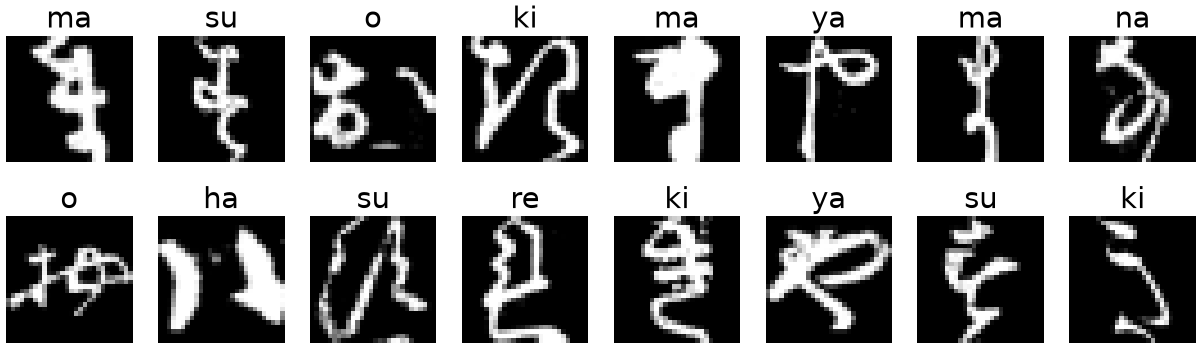
\includegraphics[width=13cm]{fig01_muestras.png}
    \caption{Primeras dieciséis imágenes de entrenamiento de KMNIST con su clase}
    \label{fig:muestras}
\end{figure}

\subsection{Arquitectura propuesta}

El enunciado pide al menos dos bloques de convolución con normalización por lotes y \emph{pooling}, \emph{dropout} antes de la capa final y menos de 200\,000 parámetros. La red de la Tabla~\ref{tab:arq} y la Figura~\ref{fig:arq} cumple con \nPar{} parámetros, una cuarta parte del límite. Cada componente tiene una razón. La convolución con relleno conserva el tamaño para que sea el \emph{pooling} quien decida la reducción. Los 32 y 64 filtros duplican los 16 y 32 de la red del cuaderno resuelto porque las formas de KMNIST son más variadas que las de los dígitos. La normalización por lotes va justo después de cada convolución y antes de la ReLU, el orden habitual, para estabilizar el entrenamiento con la tasa de $10^{-3}$. El \emph{dropout} de 0.3 protege la capa lineal, que concentra el \parFcPct{} por ciento de los parámetros (\parFc) y es donde más riesgo hay de memorizar.

\begin{table}[!htb]
    \centering
    \caption{Capas de la red propuesta. Las convoluciones usan relleno de un píxel y conservan el tamaño}
    \label{tab:arq}
    \footnotesize
    \begin{tabular}{llr}
        \toprule
        \textbf{Bloque} & \textbf{Capa} & \textbf{Parámetros} \\
        \midrule
        \multirow{2}{*}{1} & Convolución 3 por 3, 32 filtros, salida 32 por 28 por 28 & \parConv \\
                           & Normalización por lotes, ReLU, max pooling 2 por 2, salida 32 por 14 por 14 & \parBn \\
        \midrule
        \multirow{2}{*}{2} & Convolución 3 por 3, 64 filtros, salida 64 por 14 por 14 & \parConvb \\
                           & Normalización por lotes, ReLU, max pooling 2 por 2, salida 64 por 7 por 7 & \parBnb \\
        \midrule
        \multirow{2}{*}{Salida} & Aplanar, 3\,136, y dropout 0.3 & 0 \\
                                & Lineal 3\,136 a 10 & \parFc \\
        \midrule
         & Total & \nPar \\
        \bottomrule
    \end{tabular}
\end{table}

\begin{figure}[!htb]
    \centering
    \begin{tikzpicture}[node distance=0.35cm]
        \node[capa, fill=cEntrada] (e) {Entrada\\1 por 28 por 28};
        \node[capa, fill=cConv, right=of e] (c1) {Conv 3 por 3\\32 filtros};
        \node[capa, fill=cConv, right=of c1] (b1) {Norm. lotes\\ReLU};
        \node[capa, fill=cPool, right=of b1] (p1) {Max pooling\\2 por 2};
        \node[capa, fill=cConv, below=1.0cm of p1] (c2) {Conv 3 por 3\\64 filtros};
        \node[capa, fill=cConv, left=of c2] (b2) {Norm. lotes\\ReLU};
        \node[capa, fill=cPool, left=of b2] (p2) {Max pooling\\2 por 2};
        \node[capa, fill=cReg, left=of p2] (dr) {Aplanar 3\,136\\Dropout 0.3};
        \node[capa, fill=cDensa, below=0.45cm of dr] (o) {Lineal 10\\logits};
        \draw[flecha] (e) -- (c1); \draw[flecha] (c1) -- (b1); \draw[flecha] (b1) -- (p1);
        \draw[flecha] (p1) -- (c2); \draw[flecha] (c2) -- (b2); \draw[flecha] (b2) -- (p2); \draw[flecha] (p2) -- (dr); \draw[flecha] (dr) -- (o);
        \node[tensor, above=0.02cm of c1] {32 por 28 por 28};
        \node[tensor, above=0.02cm of p1] {32 por 14 por 14};
        \node[tensor, below=0.02cm of c2] {64 por 14 por 14};
        \node[tensor, below=0.02cm of p2] {64 por 7 por 7};
    \end{tikzpicture}
    \caption{Red propuesta, \nPar{} parámetros. Junto a cada bloque va el tamaño de su salida}
    \label{fig:arq}
\end{figure}

\subsection{Entrenamiento, evaluación y aumento}

El bucle de entrenamiento sigue los cinco pasos de cada iteración, borrar los gradientes, propagar el lote, calcular la entropía cruzada, retropropagar y actualizar con Adam a tasa $10^{-3}$, con lotes de 64 imágenes y \epocas{} épocas. La prueba se usa una sola vez. El aumento desplaza cada lote un número entero aleatorio de píxeles entre $-2$ y $2$ en cada eje con \texttt{torch.roll}, lo que sale por un borde entra por el opuesto. La comparación con y sin aumento se hace con la misma semilla y las mismas épocas, y se repite con las semillas 42, 43 y 44 para separar el efecto del ruido.

\section{Resultados}

\subsection{Exploración del conjunto}

Las diez clases tienen entre \conteoMin{} y \conteoMax{} imágenes de entrenamiento, una diferencia menor al 2 por ciento, así que el conjunto está balanceado y la exactitud global es una medida fiable. No hace falta ponderar las clases ni remuestrear.

\subsection{Entrenamiento}

La Tabla~\ref{tab:epocas} y la Figura~\ref{fig:curvas} muestran las \epocas{} épocas. La pérdida de entrenamiento baja de \lossA{} a \lossZ{} y la exactitud de validación sube de \vaccA{} a \vaccZ{} por ciento, con su máximo de \vaccMax{} en la época \epVaccMax. Entrenamiento y validación terminan juntos, \accZ{} y \vaccZ{} por ciento, sin brecha de sobreajuste.

\begin{table}[!htb]
    \centering
    \caption{Pérdida y exactitud por época de la red propuesta. La exactitud está en porcentaje}
    \label{tab:epocas}
    \footnotesize
    \begin{tabular}{c S[table-format=1.4] S[table-format=2.2] S[table-format=1.4] S[table-format=2.2]}
        \toprule
         & \multicolumn{2}{c}{\textbf{Entrenamiento}} & \multicolumn{2}{c}{\textbf{Validación}} \\
        \cmidrule(lr){2-3} \cmidrule(lr){4-5}
        \textbf{Época} & {\textbf{Pérdida}} & {\textbf{Exactitud}} & {\textbf{Pérdida}} & {\textbf{Exactitud}} \\
        \midrule
\filasEpocas
        \bottomrule
    \end{tabular}
\end{table}

\begin{figure}[!htb]
    \centering
    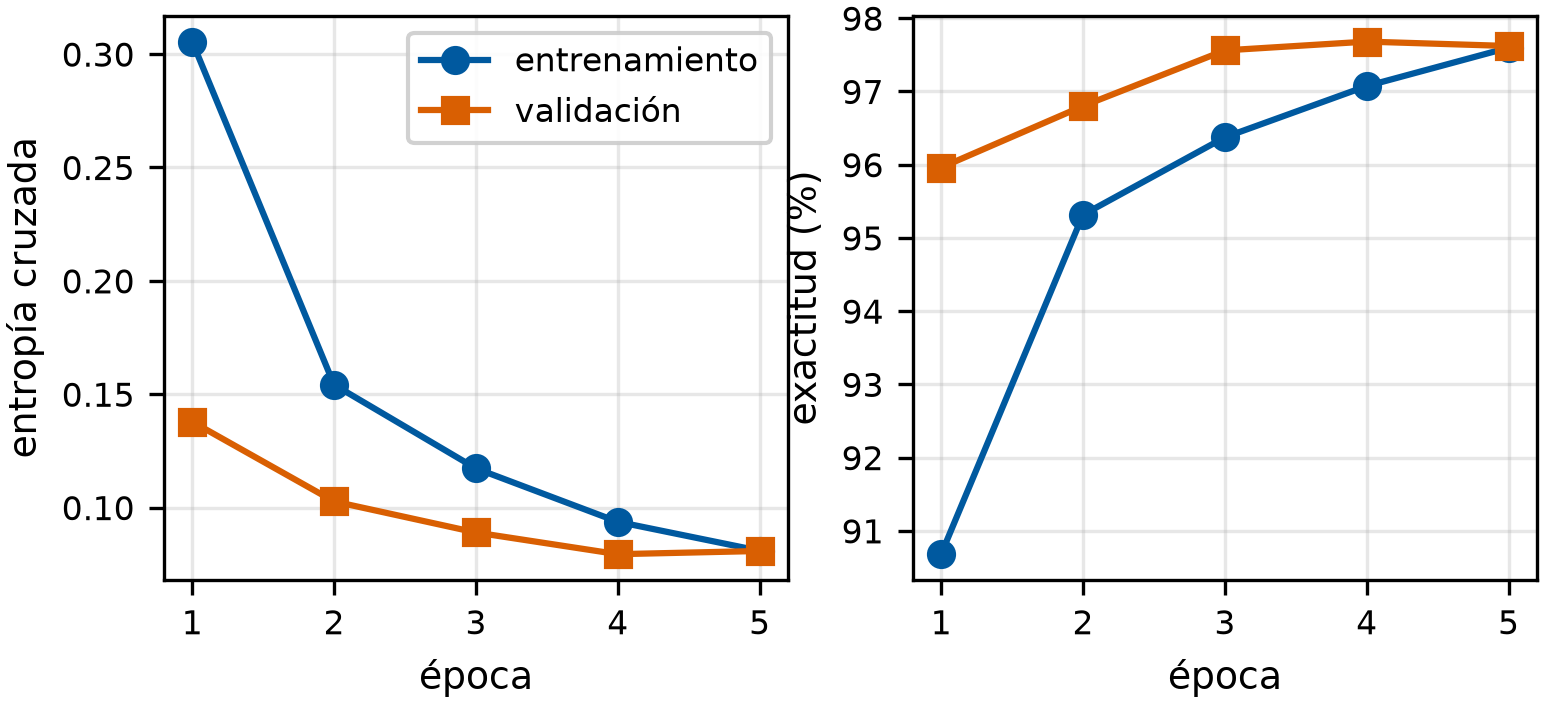
\includegraphics[width=15cm]{fig02_curvas.png}
    \caption{Pérdida y exactitud por época de la red propuesta en KMNIST}
    \label{fig:curvas}
\end{figure}

\subsection{Evaluación en prueba}

La exactitud en prueba es \accTe{} por ciento, \erroresTe{} errores de \nTe{}, con pérdida \perdTe, \brecha{} puntos por debajo de la validación. La Figura~\ref{fig:confusion} muestra la matriz de confusión y la Tabla~\ref{tab:clases} el acierto por clase, que va de \accPeor{} por ciento en \parReal{} a \accMejor{} en \claseMejor. El par más confundido es \parReal{} tomado por \parPred, \parN{} de las \parTotal{} imágenes de \parReal. La columna \colMax{} recibe \colMaxN{} errores de casi todas las clases, el \colMaxPct{} por ciento de todos los errores. La Figura~\ref{fig:par} muestra cinco imágenes del par confundido junto a imágenes bien clasificadas de las dos clases.

\begin{figure}[!htb]
    \centering
    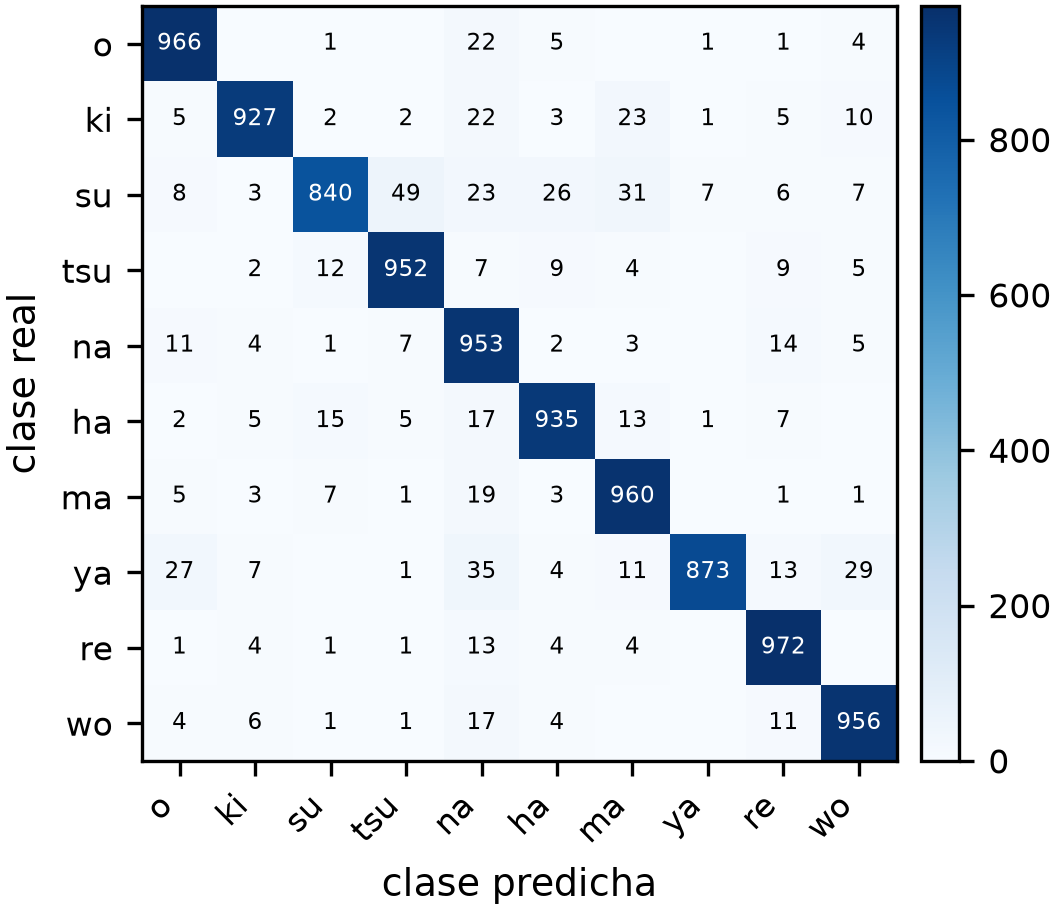
\includegraphics[width=9cm]{fig03_confusion.png}
    \caption{Matriz de confusión sobre las \nTe{} imágenes de prueba}
    \label{fig:confusion}
\end{figure}

\begin{table}[!htb]
    \centering
    \caption{Acierto por clase en prueba. El acierto es la fracción de imágenes de la clase bien clasificadas y la precisión la fracción de predicciones de esa clase que eran correctas}
    \label{tab:clases}
    \footnotesize
    \begin{tabular}{l S[table-format=4.0] S[table-format=4.0] S[table-format=2.1] S[table-format=2.1]}
        \toprule
        \textbf{Clase} & {\textbf{Imágenes}} & {\textbf{Aciertos}} & {\textbf{Acierto (\%)}} & {\textbf{Precisión (\%)}} \\
        \midrule
\filasPorClase
        \bottomrule
    \end{tabular}
\end{table}

\begin{figure}[!htb]
    \centering
    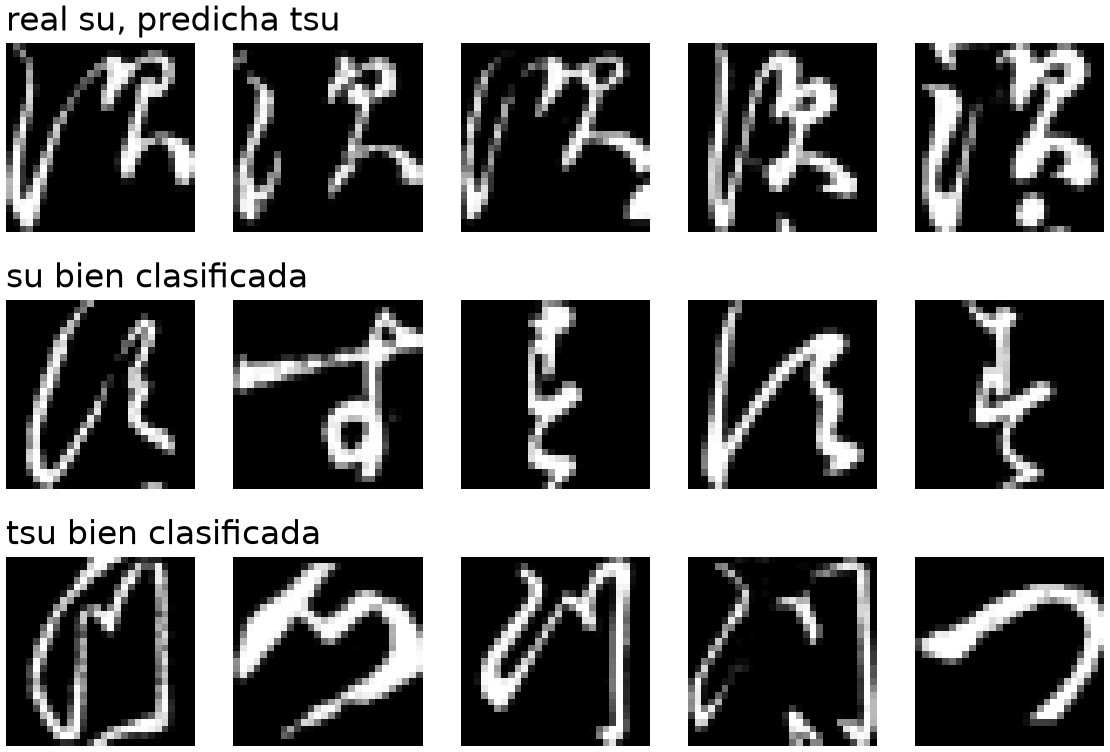
\includegraphics[width=12cm]{fig04_par.png}
    \caption{Arriba, imágenes de \parReal{} que la red tomó por \parPred. En medio y abajo, imágenes de \parReal{} y de \parPred{} bien clasificadas}
    \label{fig:par}
\end{figure}

\subsection{Aumento de datos}

La Figura~\ref{fig:aumento} muestra el efecto del desplazamiento sobre cuatro imágenes. La Tabla~\ref{tab:aumento} y la Figura~\ref{fig:barras} resumen tres semillas con \epocas{} épocas cada una. Con aumento la exactitud de entrenamiento baja \augDifTr{} puntos, la de validación cambia \augDifVal{} y la de prueba \augDifTe, las dos últimas dentro de la desviación entre semillas. La brecha entre validación y entrenamiento pasa de \augBrechaSin{} a \augBrechaCon{} puntos.

\begin{figure}[!htb]
    \centering
    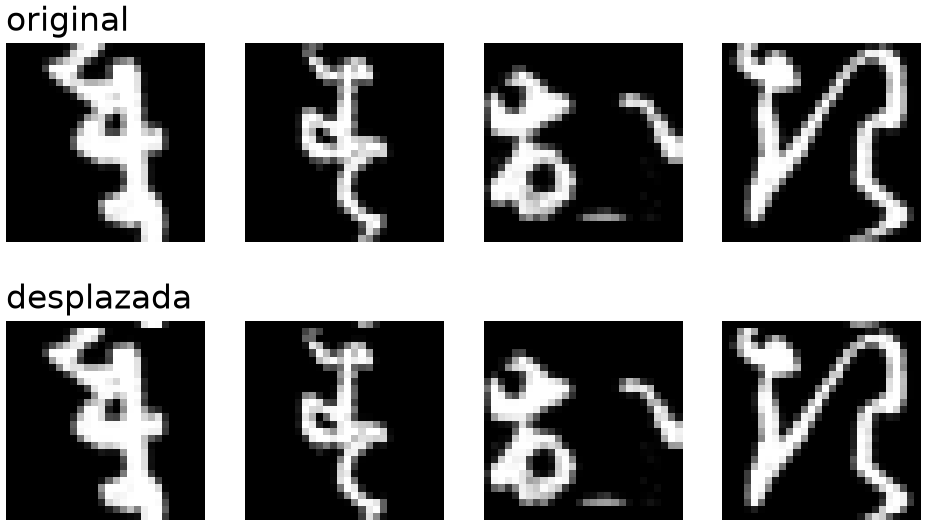
\includegraphics[width=10cm]{fig05_aumento.png}
    \caption{Cuatro imágenes de entrenamiento antes y después del desplazamiento aleatorio}
    \label{fig:aumento}
\end{figure}

\begin{table}[!htb]
    \centering
    \caption{Exactitud en porcentaje, media y desviación de las semillas 42, 43 y 44 con \epocas{} épocas}
    \label{tab:aumento}
    \footnotesize
    \begin{tabular}{l c c c}
        \toprule
         & \textbf{Entrenamiento} & \textbf{Validación} & \textbf{Prueba} \\
        \midrule
        Sin aumento & $\augSinTr \pm \augSinTrSd$ & $\augSinVal \pm \augSinValSd$ & $\augSinTe \pm \augSinTeSd$ \\
        Con aumento & $\augConTr \pm \augConTrSd$ & $\augConVal \pm \augConValSd$ & $\augConTe \pm \augConTeSd$ \\
        \bottomrule
    \end{tabular}
\end{table}

\begin{figure}[!htb]
    \centering
    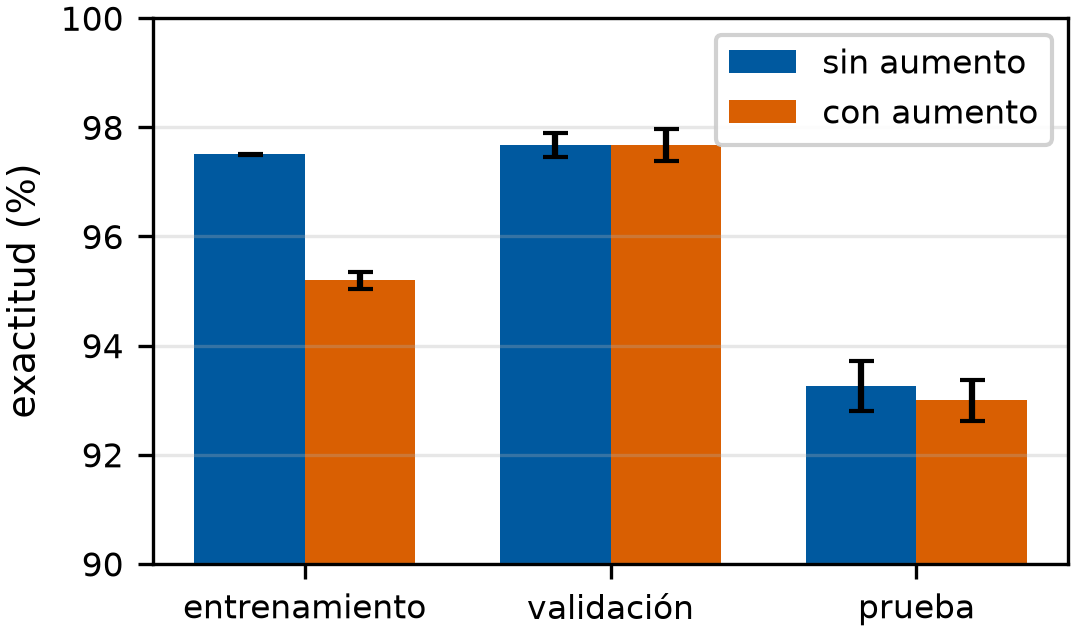
\includegraphics[width=10cm]{fig06_aumento_barras.png}
    \caption{Exactitud media de las tres semillas con y sin aumento. Las barras de error son la desviación entre semillas}
    \label{fig:barras}
\end{figure}

\section{Análisis}

\subsection{Por qué cada componente de la red}

La pregunta del paso 2 era qué se esperaba de cada componente. La convolución aporta filtros que se reutilizan en toda la imagen, y con 32 y 64 de ellos la red tiene margen para las variantes de forma de KMNIST. La normalización por lotes hizo lo que se esperaba, la red llegó a \vaccA{} por ciento de validación en la primera época con la tasa de $10^{-3}$, sin ningún ajuste de la tasa. El \emph{pooling} redujo las 3\,136 características de la capa lineal a una cantidad manejable, y aun así esa capa concentra el \parFcPct{} por ciento de los parámetros, lo que justifica el \emph{dropout} delante de ella. La Tabla~\ref{tab:epocas} muestra que la combinación funcionó, entrenamiento y validación avanzan juntos y la pérdida de validación baja en cada época.

\subsection{La brecha entre validación y prueba}

La validación termina en \vaccZ{} por ciento y la prueba en \accTe, \brecha{} puntos menos. No es sobreajuste, porque el entrenamiento y la validación coinciden y el \emph{dropout} está activo. La validación es una muestra al azar del mismo conjunto de entrenamiento, escrita por las mismas manos y con las mismas formas, mientras que la prueba de KMNIST proviene de otros documentos. Una validación tomada del entrenamiento no puede anticipar esa diferencia, y por eso la prueba se reserva para una sola medición final. En MNIST la brecha fue de dos décimas de punto porque sus dígitos de prueba se parecen mucho a los de entrenamiento. Esta diferencia entre los dos conjuntos es la lección más clara del taller.

\subsection{Por qué se confunden su y tsu}

El par más frecuente es \parReal{} tomado por \parPred. La Figura~\ref{fig:par} lo explica. La clase \parReal{} reúne varias formas antiguas del carácter, y las cinco imágenes mal clasificadas comparten dos trazos verticales largos con un lazo, mientras que las de \parReal{} bien clasificadas muestran formas más compactas y distintas entre sí. Las imágenes de \parPred{} bien clasificadas tienen también trazos verticales largos que se cierran, así que la variante alargada de \parReal{} cae en el territorio visual de \parPred. La red no falla por un defecto del entrenamiento sino porque una misma clase contiene formas que se parecen más a otra clase que entre sí. La columna \colMax{} con el \colMaxPct{} por ciento de los errores muestra otra cosa, la red usa \colMax{} como respuesta por defecto ante formas que no reconoce bien, probablemente porque sus trazos curvos y sueltos se parecen a fragmentos de muchos otros caracteres.

\subsection{Qué hizo y qué no hizo el aumento de datos}

El aumento no mejoró la exactitud de prueba ni la de validación. Las diferencias de \augDifVal{} y \augDifTe{} puntos están dentro de la desviación entre semillas, así que no se puede afirmar un cambio en ningún sentido. Lo que sí cambió es la brecha, que pasó de \augBrechaSin{} a \augBrechaCon{} puntos porque el entrenamiento cayó \augDifTr{} puntos. Es el comportamiento esperado de un regularizador, la red ve imágenes más difíciles de las que después evalúa. Pero un regularizador solo ayuda cuando hay sobreajuste que corregir, y en \epocas{} épocas no lo había. Hay además dos razones para que no ayude en la prueba. El \emph{pooling} ya tolera desplazamientos de uno o dos píxeles, de modo que la red no necesitaba verlos durante el entrenamiento. Y los errores de prueba no vienen de la posición del carácter sino de su forma, como muestra el par \parReal{} y \parPred, y un desplazamiento no cambia la forma. Si se quisiera cerrar la brecha de prueba haría falta un aumento que cambie la forma, por ejemplo pequeñas rotaciones o deformaciones del trazo, y más épocas para que el regularizador tenga algo que corregir.

\section{Conclusiones}

La red propuesta de dos bloques con normalización por lotes y \emph{dropout} alcanza \vaccZ{} por ciento de validación y \accTe{} de prueba en KMNIST con \nPar{} parámetros, y cumple todas las restricciones del enunciado con las diez verificaciones en \texttt{[OK]}.

La brecha de \brecha{} puntos entre validación y prueba no es sobreajuste. Las curvas de entrenamiento y validación coinciden, y la diferencia viene de que la prueba de KMNIST proviene de otros documentos. Una validación tomada del entrenamiento no puede detectar eso.

El error dominante, \parReal{} tomado por \parPred{} en \parN{} de \parTotal{} imágenes, nace de una clase que agrupa formas de escritura muy distintas, y la columna \colMax{} concentra el \colMaxPct{} por ciento de los errores como respuesta por defecto de la red.

El aumento por desplazamiento de dos píxeles no cambió la exactitud de validación ni de prueba con tres semillas, y solo redujo la de entrenamiento. En \epocas{} épocas no había sobreajuste que corregir, el \emph{pooling} ya tolera esos desplazamientos y los errores son de forma y no de posición.

Repetir el experimento con tres semillas fue necesario. Con una sola, la primera comparación daba al aumento una ventaja de medio punto en prueba que desapareció al promediar.

\section{Referencias}
\begin{itemize}
    \item Clanuwat, T., Bober-Irizar, M., Kitamoto, A., Lamb, A., Yamamoto, K., \& Ha, D. (2018). Deep learning for classical Japanese literature. \textit{NeurIPS Workshop on Machine Learning for Creativity and Design}.
    \item Ioffe, S., \& Szegedy, C. (2015). Batch normalization: Accelerating deep network training by reducing internal covariate shift. \textit{International Conference on Machine Learning}.
    \item Srivastava, N., Hinton, G., Krizhevsky, A., Sutskever, I., \& Salakhutdinov, R. (2014). Dropout: A simple way to prevent neural networks from overfitting. \textit{Journal of Machine Learning Research}, 15, 1929--1958.
    \item Kingma, D. P., \& Ba, J. (2015). Adam: A method for stochastic optimization. \textit{International Conference on Learning Representations}.
    \item Paszke, A. et al. (2019). PyTorch: An imperative style, high-performance deep learning library. \textit{Advances in Neural Information Processing Systems}, 32.
\end{itemize}

\appendix
\section{Código de los bloques completados}
\label{anexo:codigo}

Se reproducen los cinco bloques \texttt{TODO} tal como quedaron en el cuaderno entregado, entre las marcas que usa el docente.

\begin{lstlisting}[caption={TODO 1, imágenes por clase}]
conteo = torch.bincount(datos["y_tr"], minlength=len(clases))
\end{lstlisting}

\begin{lstlisting}[caption={TODO 2, arquitectura}]
class CNNPropia(nn.Module):
    def __init__(self, p_drop=0.3):
        super().__init__()
        self.conv1 = nn.Conv2d(1, 32, kernel_size=3, padding=1)     # 28 -> 28
        self.bn1 = nn.BatchNorm2d(32)
        self.conv2 = nn.Conv2d(32, 64, kernel_size=3, padding=1)    # 14 -> 14
        self.bn2 = nn.BatchNorm2d(64)
        self.drop = nn.Dropout(p_drop)
        self.fc = nn.Linear(64 * 7 * 7, 10)
    def forward(self, x):
        x = F.max_pool2d(F.relu(self.bn1(self.conv1(x))), 2)        # 28 -> 14
        x = F.max_pool2d(F.relu(self.bn2(self.conv2(x))), 2)        # 14 -> 7
        return self.fc(self.drop(x.flatten(1)))
\end{lstlisting}

\begin{lstlisting}[caption={TODO 3, los cinco pasos de una iteración}]
opt.zero_grad()
salida = modelo(xb)
perdida = F.cross_entropy(salida, yb)
perdida.backward()
opt.step()
\end{lstlisting}

\begin{lstlisting}[caption={TODO 4, par más confundido}]
fuera = cm.copy(); np.fill_diagonal(fuera, 0)
par = tuple(int(v) for v in np.unravel_index(np.argmax(fuera), fuera.shape))
\end{lstlisting}

\begin{lstlisting}[caption={TODO 5, desplazamiento aleatorio del lote}]
def aumentar_desplazamiento(xb, max_px=2):
    dy, dx = (int(v) for v in torch.randint(-max_px, max_px + 1, (2,)))
    return torch.roll(xb, shifts=(dy, dx), dims=(2, 3))
\end{lstlisting}

\end{document}
